We evaluate the model under a strict and a relaxed condition. Under strict evaluation an alert can be matched to an event only if there is city level location match and the forecasted event date is same as the true event date. In the relaxed evaluation, we allow the matching to happen if the alert and the GSR event are within a 300 KM radius and the forecasted event date lies within a given interval of the true event date. We try different matching intervals ranging from 0 to 7. If $x$ is the allowed interval, then a matching can happen if an alert's forecasted event date is within $+x$(upper bound) days of the GSR event and with a lower bound of $min(x,GSR Event Date - Date of Forecast)$ :
\begin{itemize}
    \item {\bf Perfomance over the months}
\end{itemize}
    Fig.~\ref{fig:monthlyqs} provides the evaluation results of the model over the months with a source level breakdown. The QS reported is the weighted average of QS of all 10 countries where the weight for a country is the number of GSR events for that country.
    Twitter has a higher QS as multiple re-tweets of mention of future events in twitter is a direct indicator of the popularity of an event as well as the intent of people to join an event. While mention of Future events in News is simply a reporting of the event not much can be understood about the popularity of the event or about the people's support for the event. 
\begin{itemize}
    \item {\bf Country-wise perfomance}
\end{itemize}
    Table~\ref{tb:sourcewisecomparison} presents the perfomance of the planned protest model (for March 2014) for each of the 10 countries of interest. It also presents a source wise breakdown.From the table it is evident that different data source prefer different countries. The News/Blogs data source produces alerts for most countries and also provides much higher recall as opposed to twitter which provides High QS but very little recall.Also News/Blogs has a higher lead-time of 4.57 days as compared to twitters 2.82.

\begin{itemize}
    \item {\bf Case Study: Venezuelan and Brazilian Protests}
\end{itemize}
The recent Venezuelan protests against President Nicolas Maduro and the Brazilian Protests during June 2013 against Bus Fare Hike were two significant protests during our period of evaluation. Fig.~\ref{fig:venezuela_feb} and Fig.~\ref{fig:brazil_june} show how well the planned protest model was able to predict the unfolding of events under both situations. Fig.~\ref{fig:venezuela_violent} showcases the ability of the model to forecast the violent events also.

\begin{itemize}
    \item {\bf Lead-Time vs Quality Trade-Off}
\end{itemize}

Fig.~\ref{fig:leadTimeVsQS} shows that the QS of the planned protest model increases with time. 

\begin{itemize}
    \item {\bf Perfomance under stringent matching Criteria}
\end{itemize}
Fig.~\ref{fig:matchinginterval} shows the perfomance of the model when the matching window is varied from 7 to 1 in steps. We can see that the model is not affected badly even under the strict matching interval of 1-day difference.

\begin{itemize}
    \item {\bf Quality Score Distribution}
\end{itemize}
The hump on the right side of the Fig.~\ref{fig:doubleHump} signifies that a majority of the planned protest alerts are high quality.

\begin{table*}[tb!]
    \small
    \centering
    \caption{\label{tb:sourcewisecomparison} Comparing forecasting accuracy of
    RSS vs Twitter}
    \begin{tabular}{|*{9}{c|}}
        \hline
        & \multicolumn{4}{ |c| }{News/Blogs} & \multicolumn{4}{ |c| }{Twitter}\\
        \hline
        Country & QS & Precision & Recall &Lead-Time & QS & Precision & Recall & Lead-Time\\
        \hline
        AR &3.14&0.32&0.69&3.94&3.52&0.78&0.14&3.14\\
        BR &3.14&0.48&0.54&5.85&0.00&0.00&0.00&0.00\\
        CL &3.06&0.91&0.67&5.40&3.52&1.00&0.23&4.29\\
        CO &2.74&0.90&0.56&7.44&3.30&1.00&0.15&2.43\\
        EC &0.00&0.00&0.00&0.00&2.32&1.00&0.06&17.00\\
        MX &2.96&0.88&0.25&3.69&3.14&1.00&0.02&1.43\\
        SV &3.22&1.00&0.03&1.0&0.00&0.00&0.00&0.00\\
        PY &3.38&1.00&0.16&9.11&3.84&1.00&0.04&11.40\\
        UY &3.24&1.00&0.29&2.40&0.00&0.00&0.00&0.00\\
        VE &3.80&1.00&0.36&3.27&3.68&0.97&0.33&2.39\\
        ALL &3.34&0.69&0.35&4.57&3.62&0.97&0.15&2.82\\
        \hline
    \end{tabular}
\end{table*}

%\begin{figure*}[t]
%    \begin{subfigure}[b]{0.3\textwidth}
%        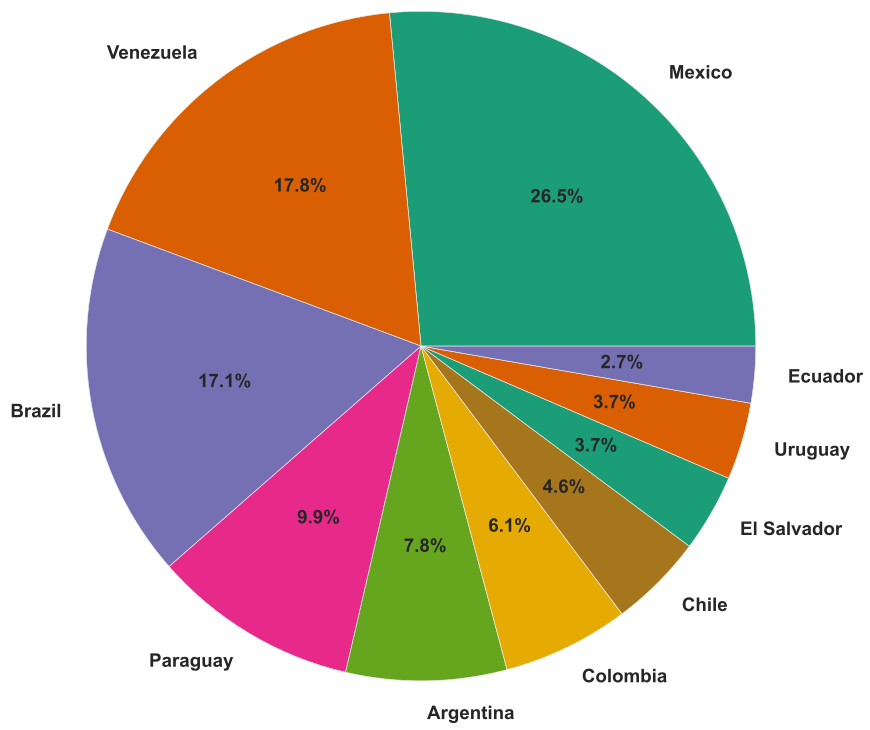
\includegraphics[width=\textwidth]{gsr_distribution}
%        \label{fig:gsrdistribution}
%        \caption{GSR Distribution From 2012-11 to 2014-03}
%    \end{subfigure}
%
%    \begin{subfigure}[b]{0.3\textwidth}
%        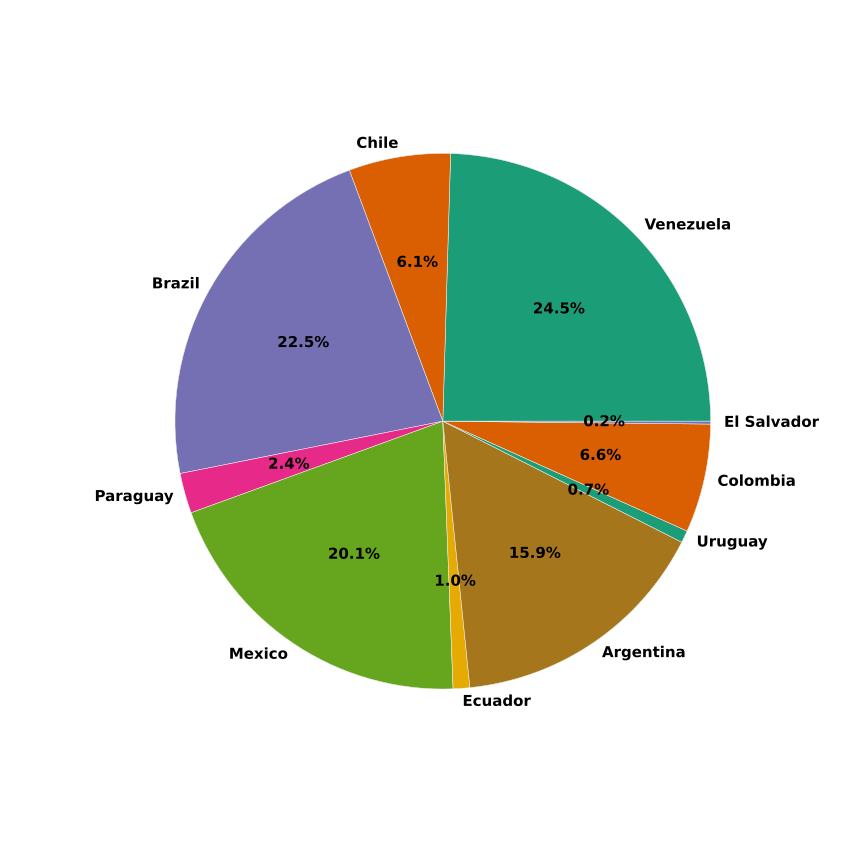
\includegraphics[width=\textwidth]{pp_dist}
%        \label{fig:ppdistribution}
%        \caption{Alerts Distribution From 2012-11 to 2014-03}
%    \end{subfigure}
%\end{figure*}
\begin{figure*}
\centering
\begin{subfigure}{.5\textwidth}
  \centering
  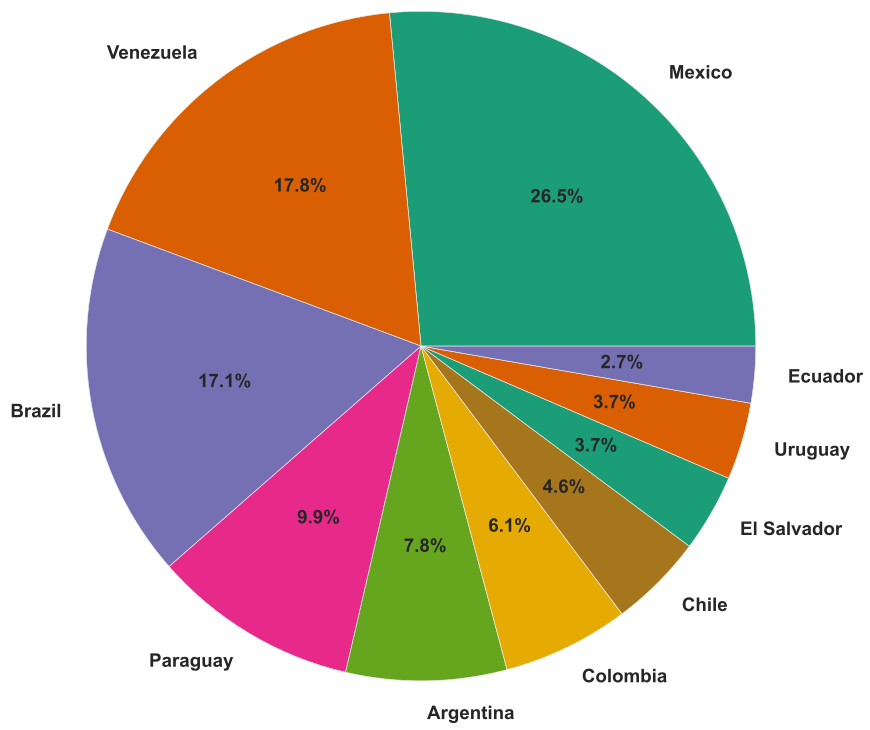
\includegraphics[width=\linewidth]{gsr_distribution}
  \caption{GSR Distribution From 2012-11 to 2014-03}
  \label{fig:gsrdistribution}
\end{subfigure}%
\begin{subfigure}{.5\textwidth}
  \centering
  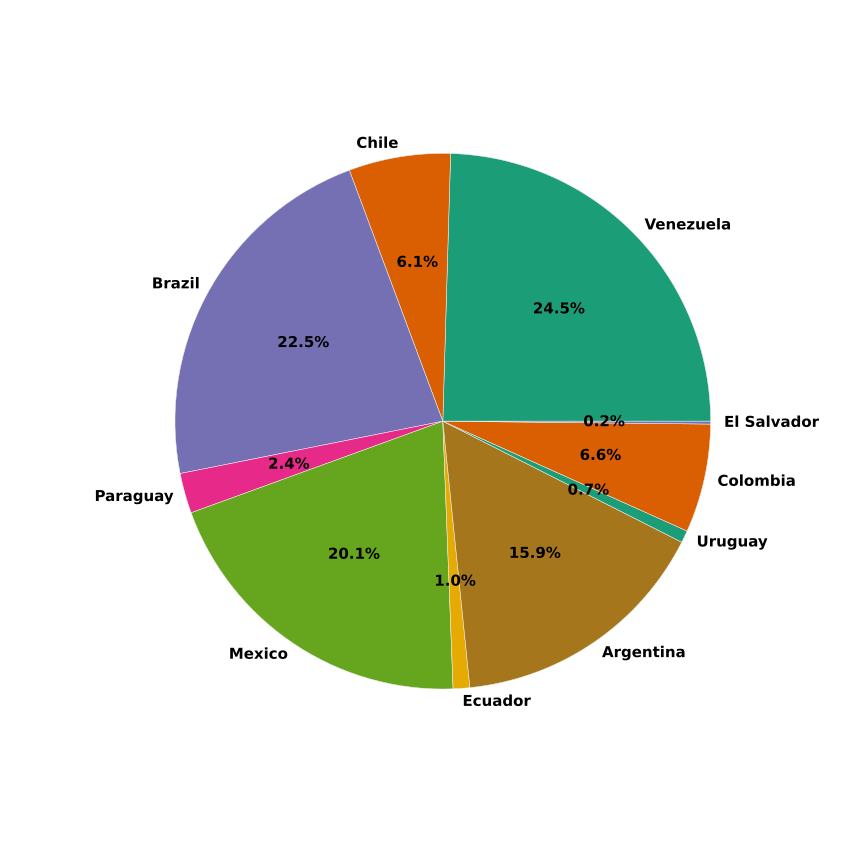
\includegraphics[width=\linewidth]{pp_dist}
  \caption{Alerts Distribution From 2012-11 to 2014-03}
  \label{fig:ppdistribution}
\end{subfigure}
\caption{Distribution of Alerts and GSR}
\label{fig:distribution}
\end{figure*}

%\begin{figure}
%    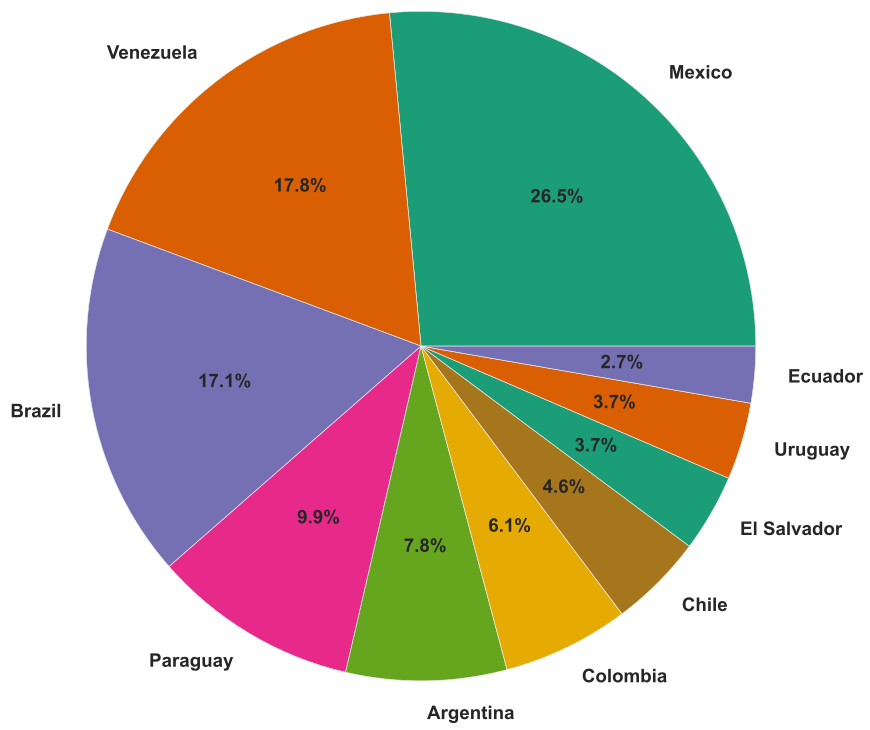
\includegraphics[width=.5\textwidth]{gsr_distribution}
%    \caption{}
%    \label{fig:gsrdistribution}
%\end{figure}
%
%\begin{figure}
%    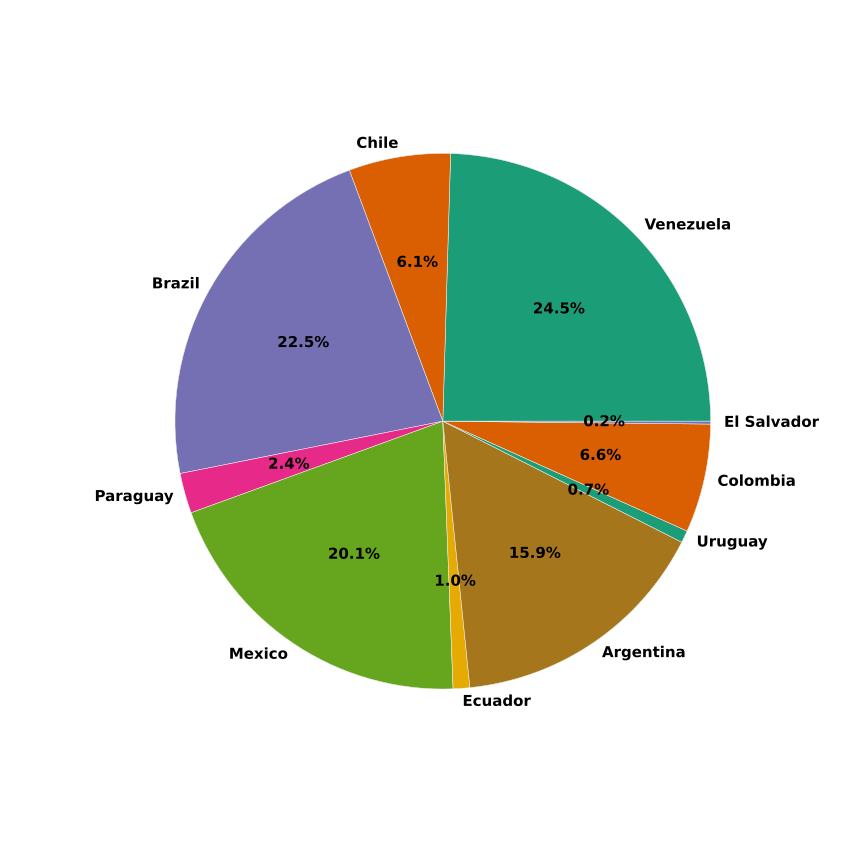
\includegraphics[width=.5\textwidth]{pp_dist}
%    \caption{Alerts Distribution From 2012-11 to 2014-03}
%    \label{fig:ppdistribution}
%\end{figure}
\begin{figure*}
\centering
\begin{subfigure}{.5\textwidth}
  \centering
  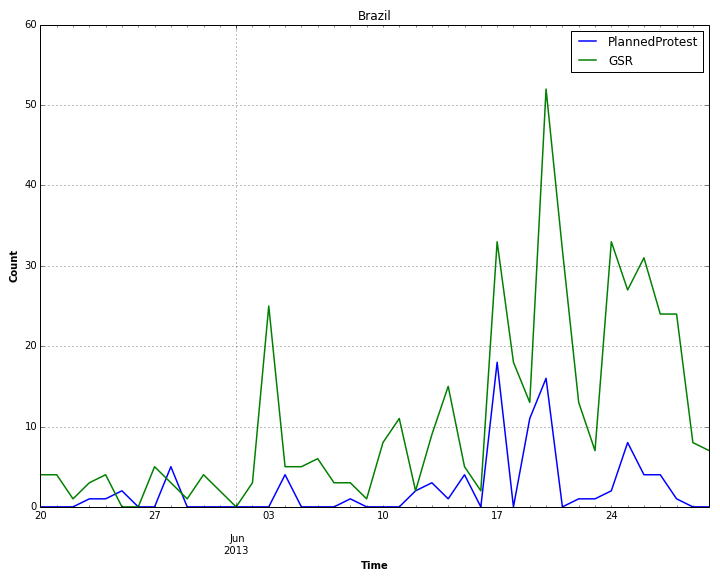
\includegraphics[width=\linewidth]{brazil_june}
  \caption{System Performance during Brazilian Spring}
  \label{fig:brazil_june}
\end{subfigure}%
\begin{subfigure}{.5\textwidth}
  \centering
  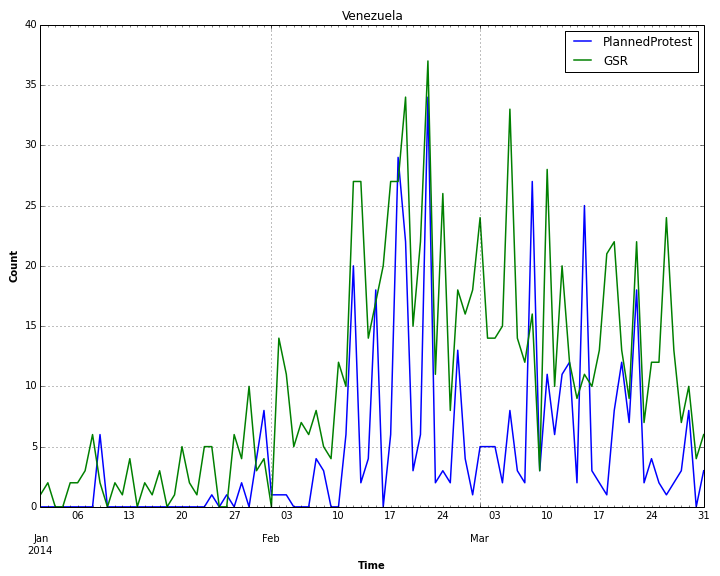
\includegraphics[width=\linewidth]{venezuela}
  \caption{Venezuelan Protests}
  \label{fig:venezuela_feb}
\end{subfigure}
\begin{subfigure}{.5\textwidth}
  \centering
  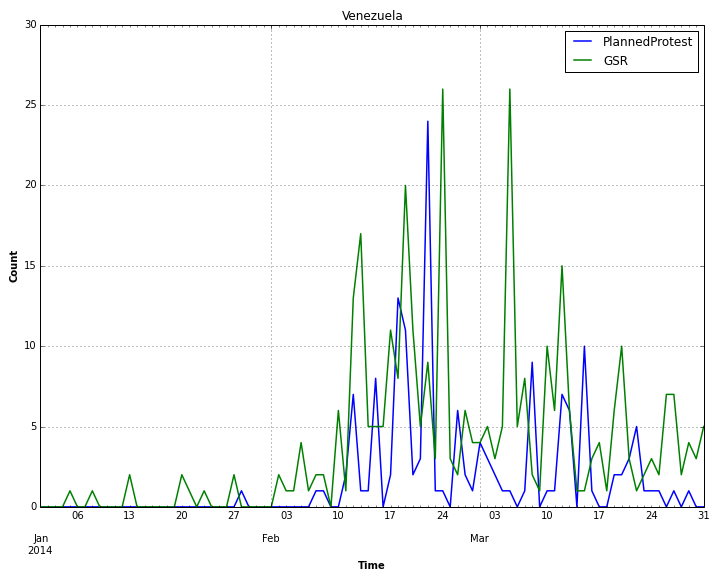
\includegraphics[width=\linewidth]{venezuela_violent}
  \caption{Venezuelan Violent Protests}
  \label{fig:venezuela_violent}
\end{subfigure}%
\begin{subfigure}{.5\textwidth}
  \centering
  
\includegraphics[width=\linewidth]{monthlyqs}
  \caption{Quality Score over the months}
  \label{fig:monthlyqs}
\end{subfigure}
\begin{subfigure}{.5\textwidth}
  \centering
  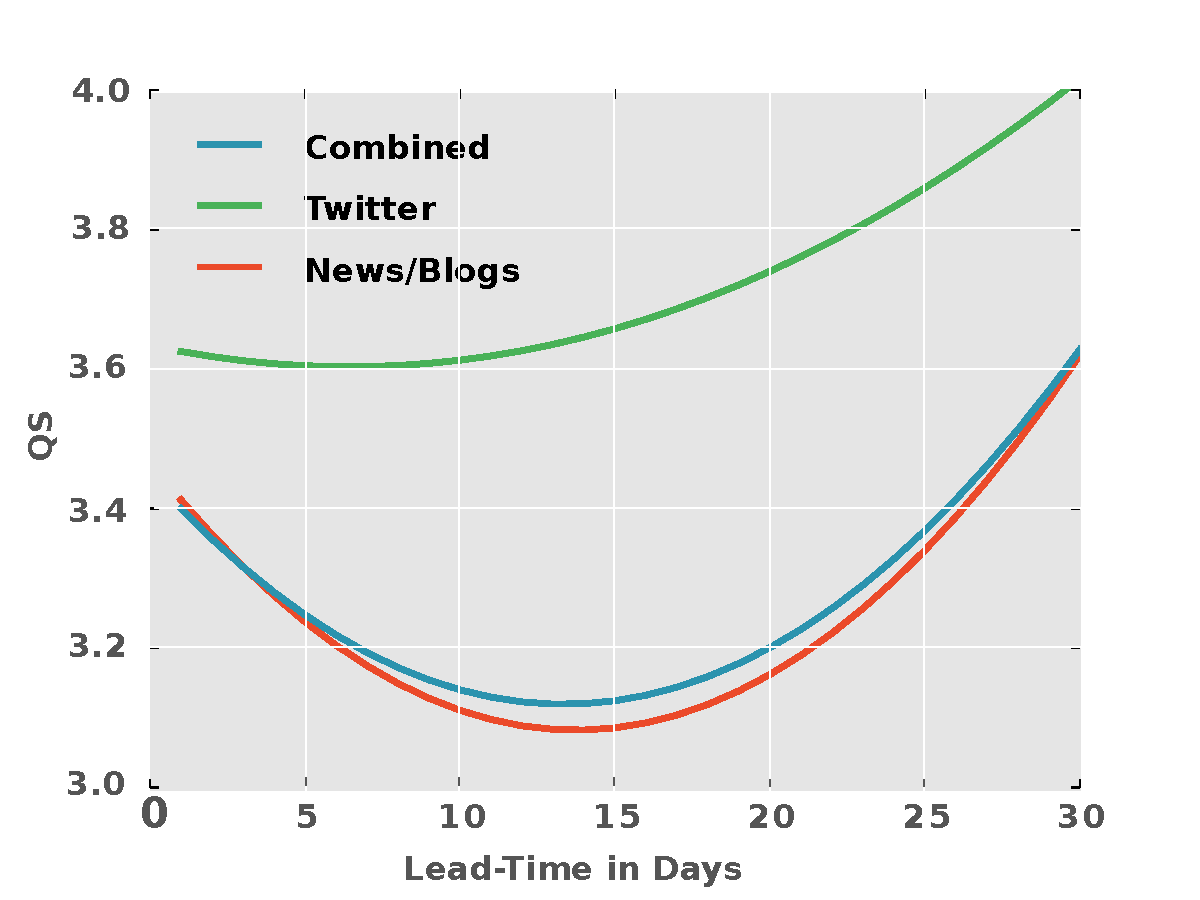
\includegraphics[width=\linewidth]{leadTimeVsQS}
  \caption{Lead-Time vs Quality Score}
  \label{fig:leadTimeVsQS}
\end{subfigure}%
\begin{subfigure}{.5\textwidth}
  \centering
  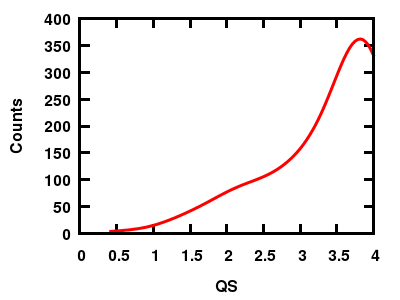
\includegraphics[width=\linewidth]{doubleHump}
  \caption{Quality Score Distribution}
  \label{fig:doubleHump}
\end{subfigure}
\begin{subfigure}{.5\textwidth}
  \centering
  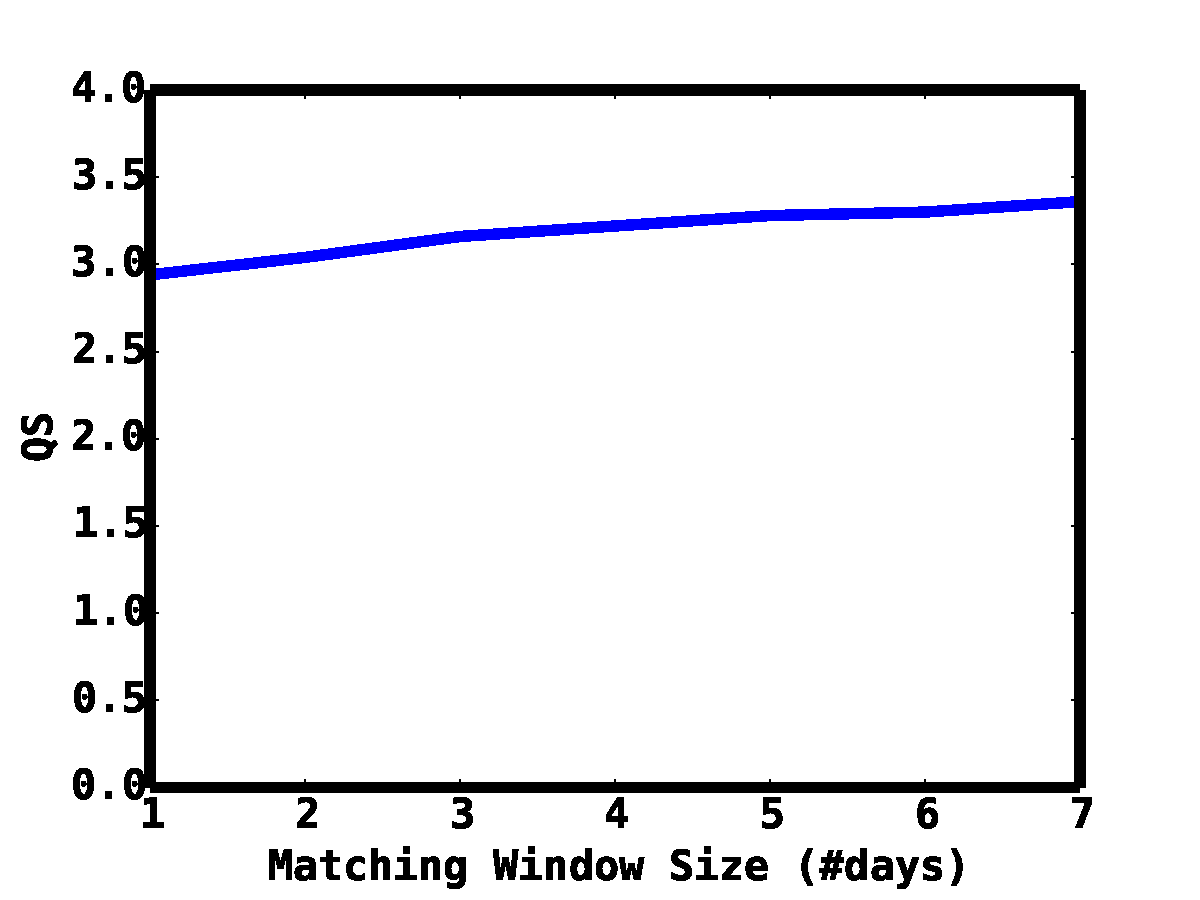
\includegraphics[width=\linewidth]{matchingwindow}
  \caption{QS vs Matching Interval Trade-Off}
  \label{fig:matchinginterval}
\end{subfigure}%
\end{figure*}

%\begin{figure}
%    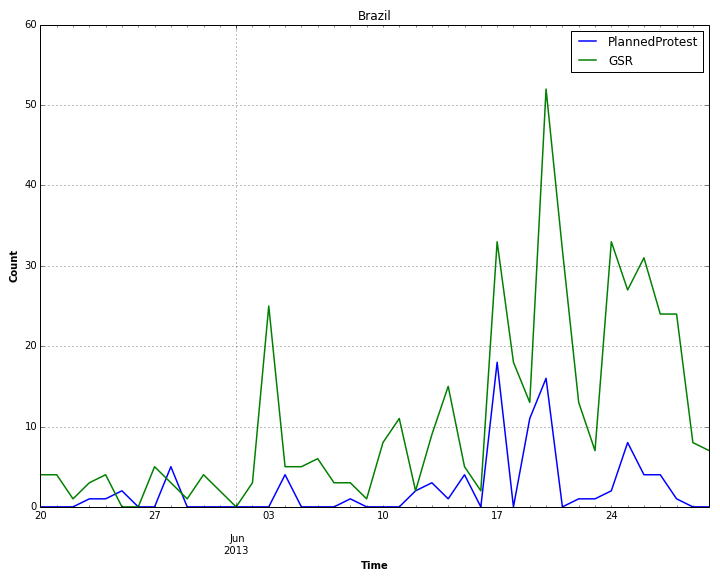
\includegraphics[width=0.5\textwidth]{brazil_june}
%    \caption{Brazil June Protests}
%    \label{fig:brazil_june}
%\end{figure}

%\begin{figure*}
%    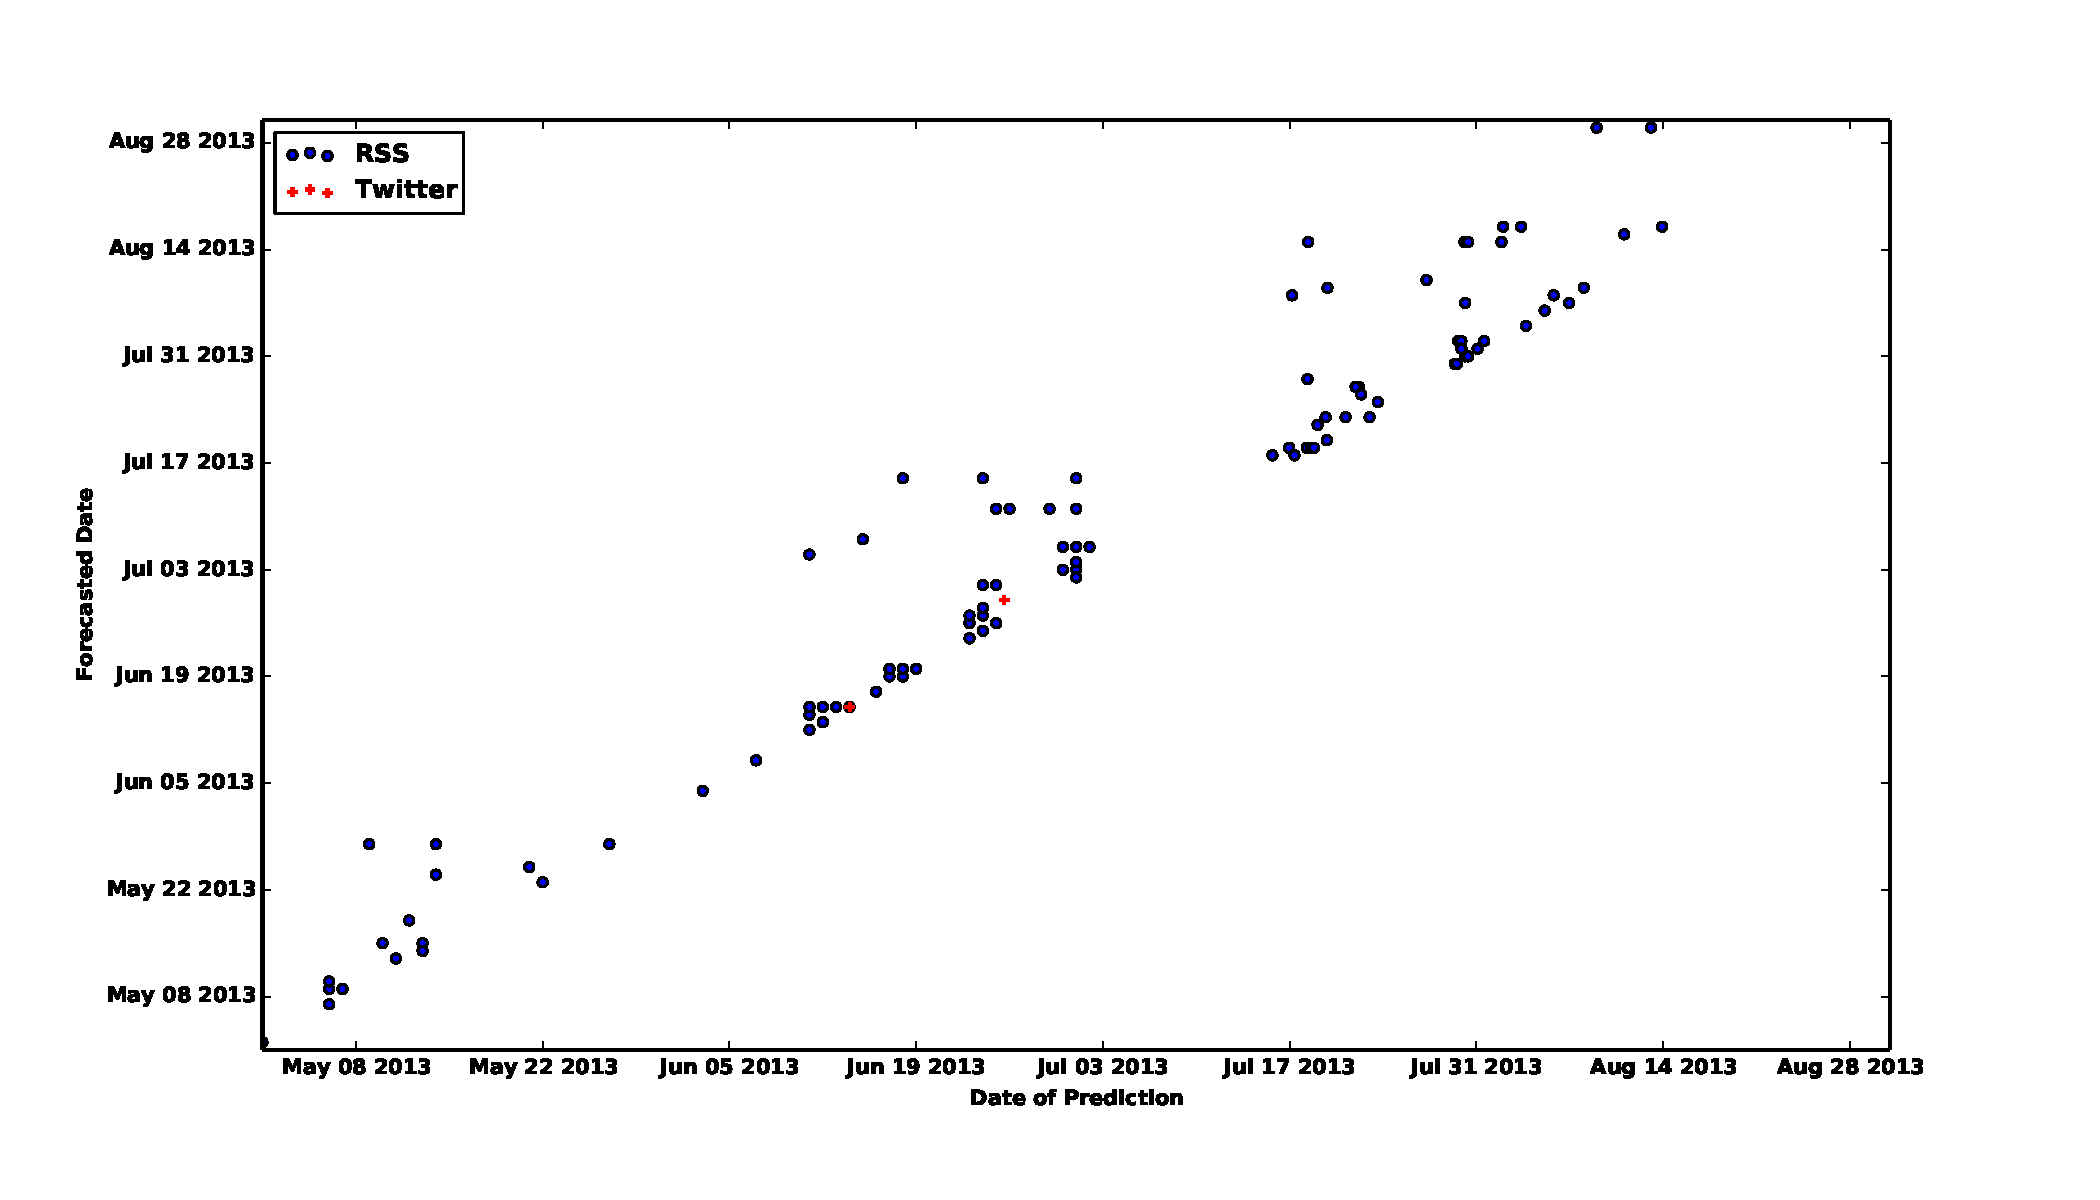
\includegraphics[width=\textwidth]{eventDateVsDate_brazil}
%    \caption{Date of Prediction vs Forecasted Date Brazil}
%    \label{fig:leadtime_brazil}
%\end{figure*}
%
%\begin{figure*}
%    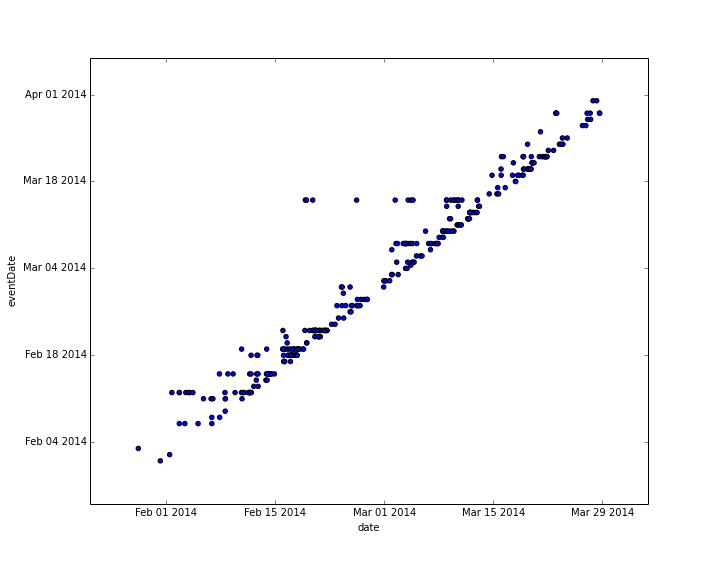
\includegraphics[width=\textwidth]{eventDateVsDate_venezuela}
%    \caption{Date of Prediction vs Forecasted Date Venezuela}
%    \label{fig:leadtime_venezuela}
%\end{figure*}

%\begin{figure}
%    
\includegraphics[width=0.5\textwidth]{monthlyqs}
%    \caption{QS over the months}
%    \label{fig:monthlyqs}
%\end{figure}
%
%\begin{figure}
%    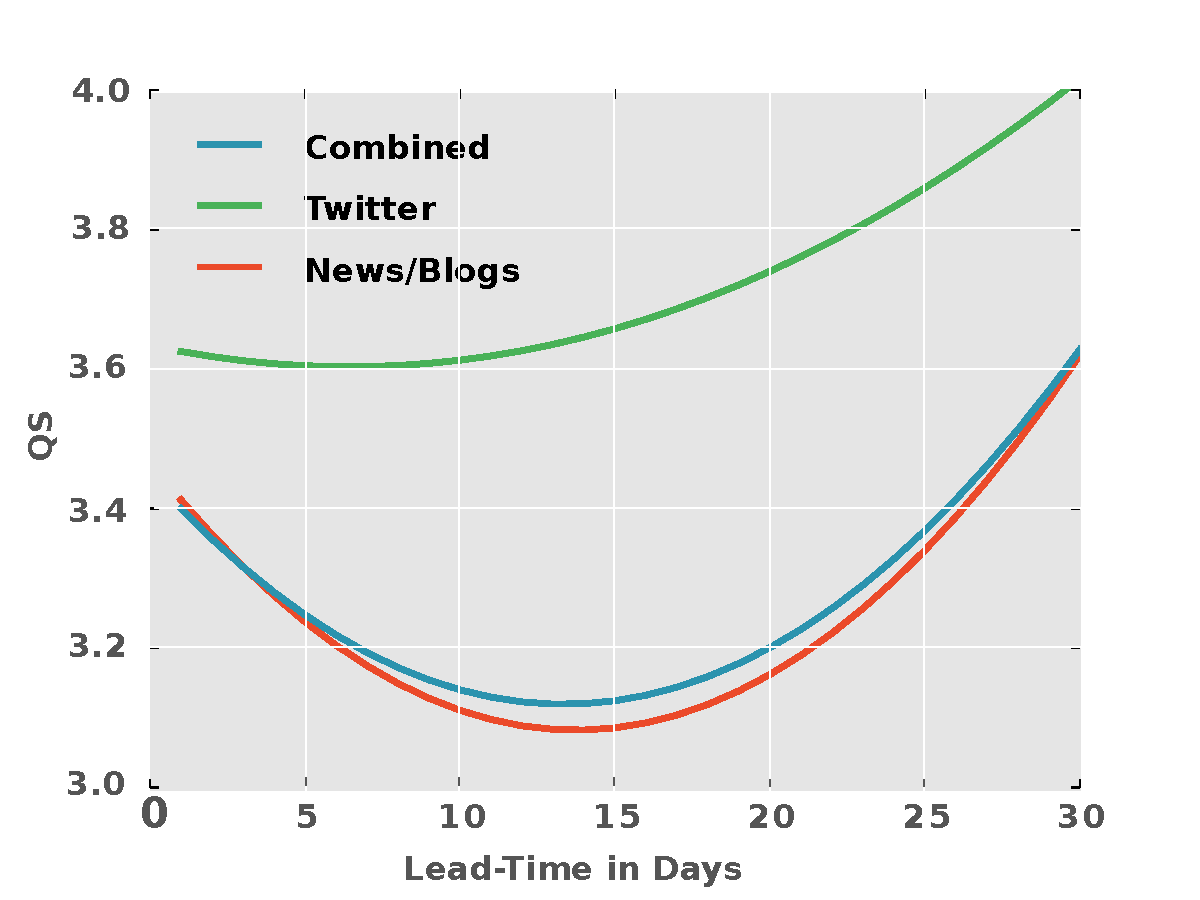
\includegraphics[width=0.5\textwidth]{leadTimeVsQS}
%    \caption{Lead-Time vs Quality Score}
%    \label{fig:leadTimeVsQS}
%\end{figure}
%
%\begin{figure}
%    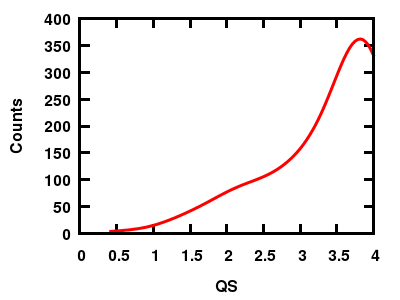
\includegraphics[width=0.5\textwidth]{doubleHump}
%    \caption{QS Distribution}
%    \label{fig:doubleHump}
%\end{figure}
%
%\begin{figure}
%    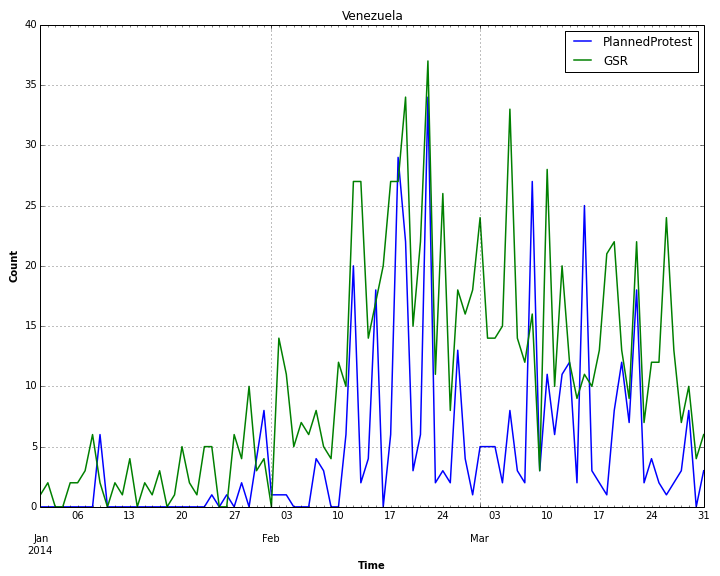
\includegraphics[width=0.5\textwidth]{venezuela}
%    \caption{Venezuelan Protests}
%    \label{fig:venezuela_feb}
%\end{figure}
%
%\begin{figure}
%    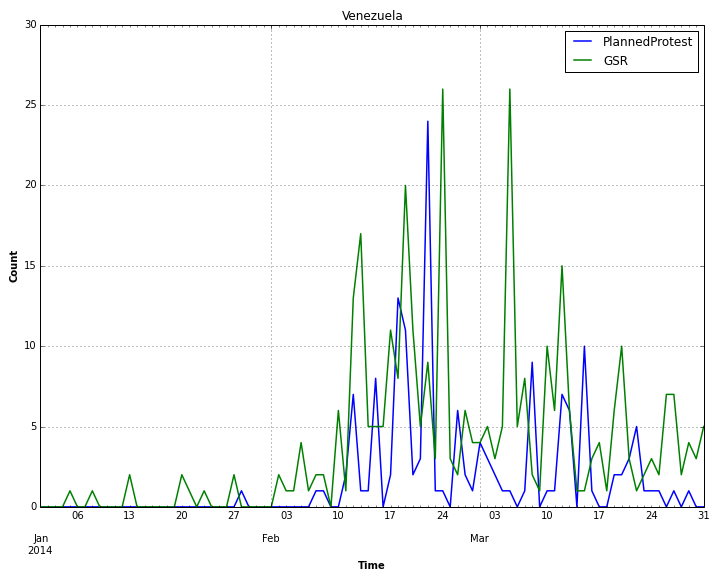
\includegraphics[width=0.5\textwidth]{venezuela_violent}
%    \caption{Venezuelan Violent Protests}
%    \label{fig:venezuela_violent}
%\end{figure}
\begin{figure}
    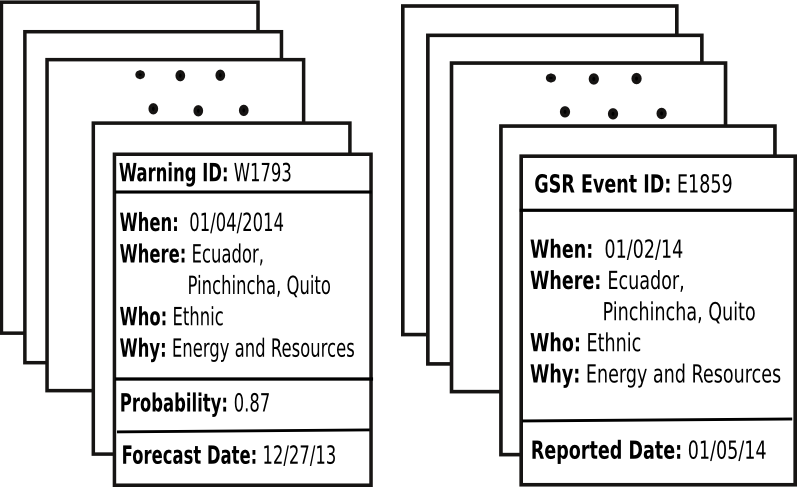
\includegraphics[width=0.5\textwidth]{alertstructure}
    \caption{Structure of an Alert}
    \label{fig:alertstructure}
\end{figure}
%\begin{figure}
%    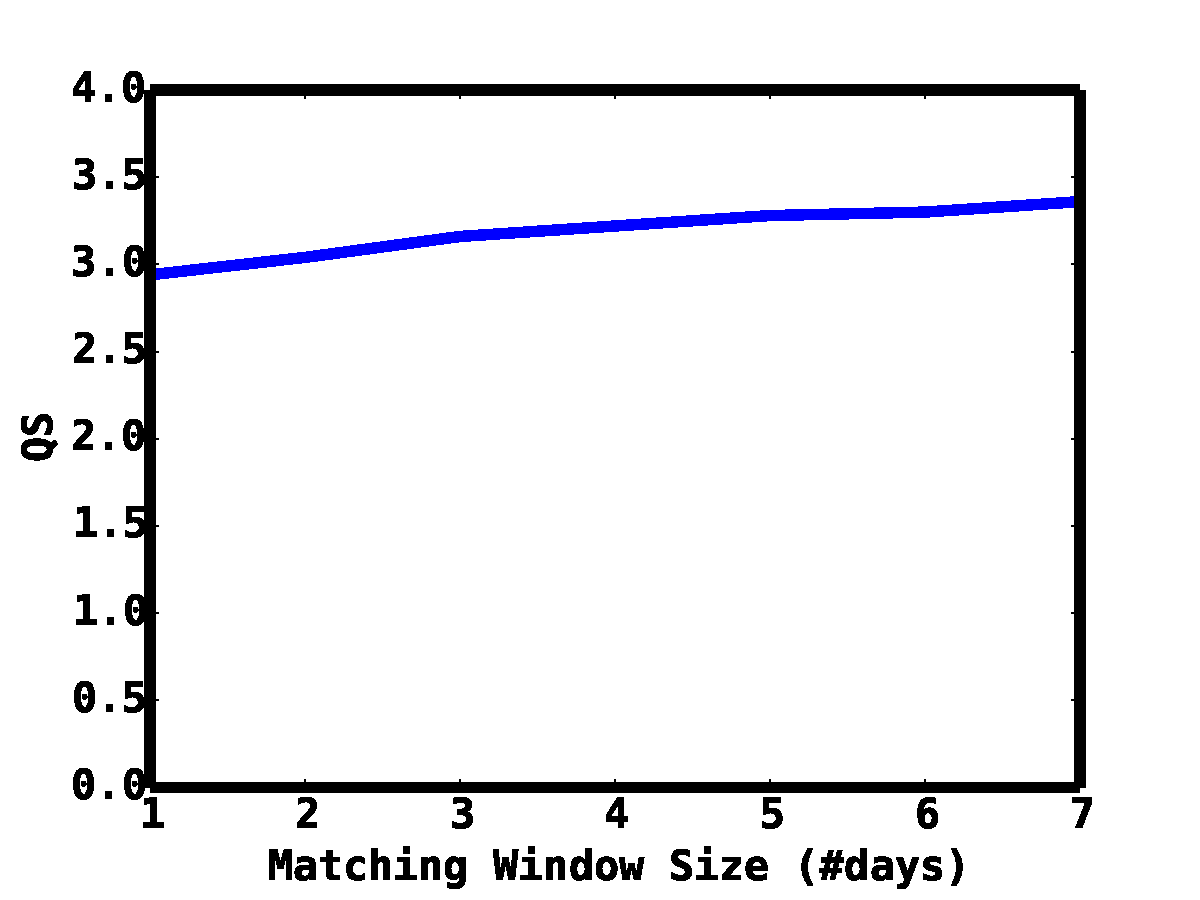
\includegraphics[width=0.5\textwidth]{matchingwindow}
%    \caption{QS vs Matching Interval Trade-Off}
%    \label{fig:matchinginterval}
%\end{figure}
\begin{figure}
    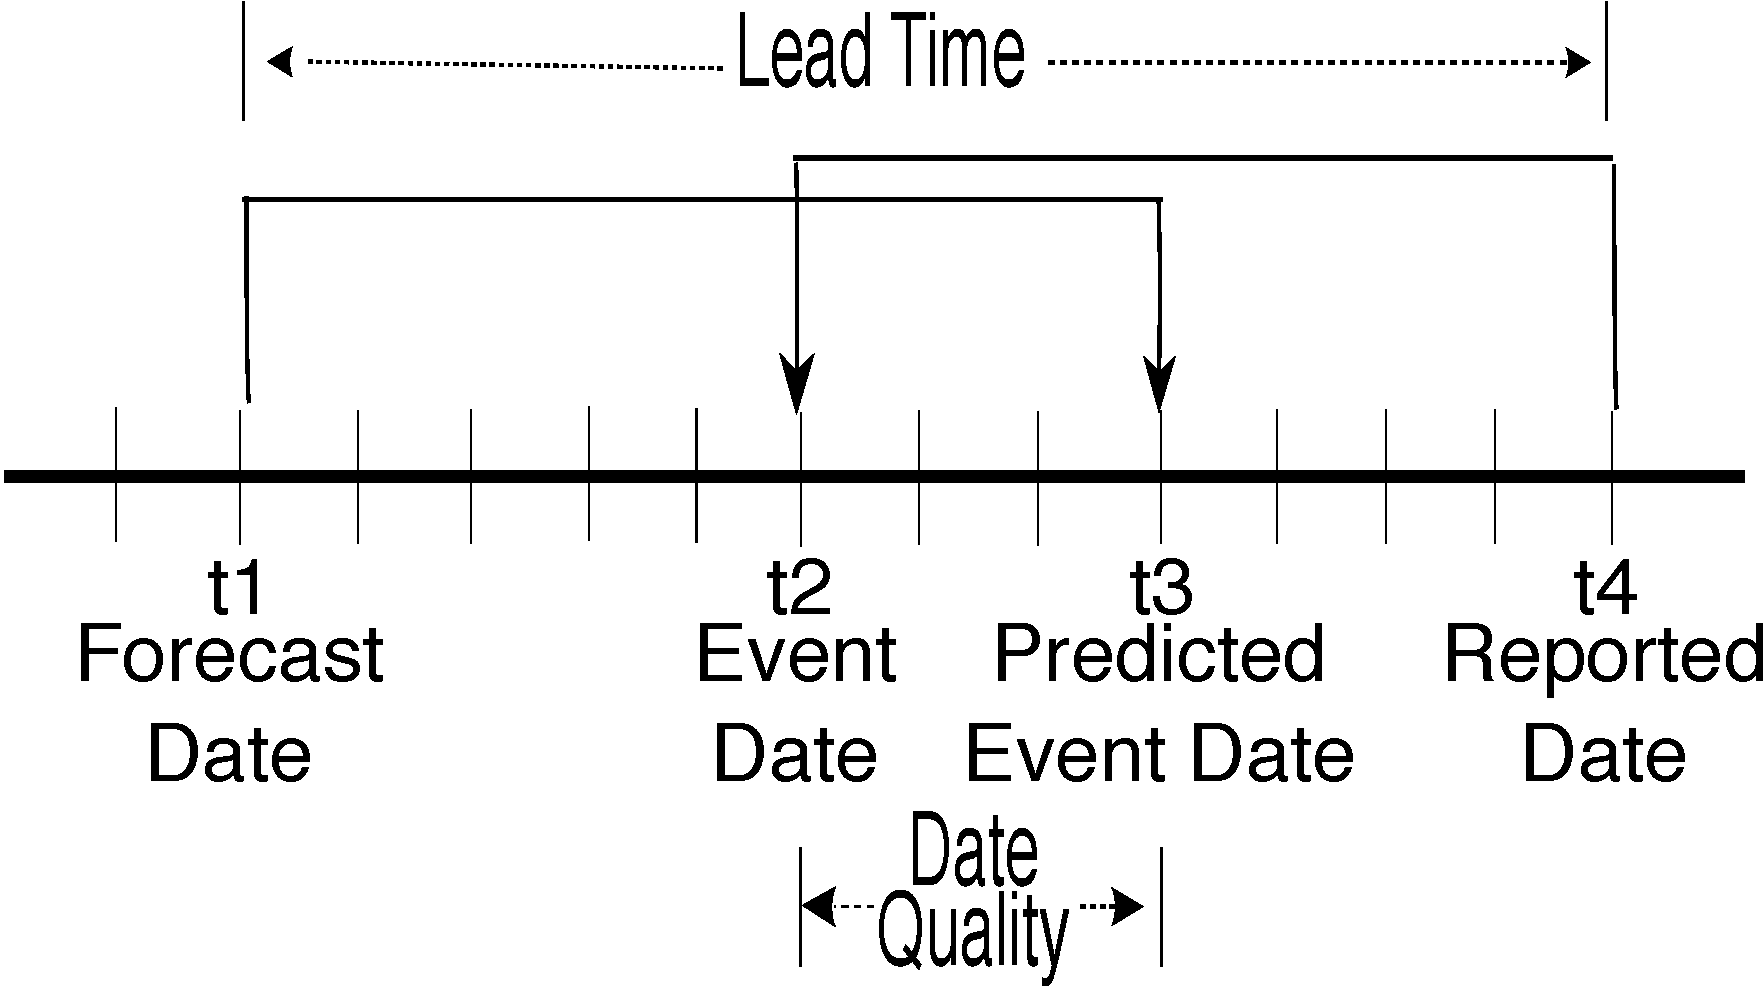
\includegraphics[width=0.5\textwidth]{timeline}
    \caption{Matching Timeline}
    \label{fig:timeline}
\end{figure}
















%\begin{figure}
%    \centering
%    \begin{subfigure}[b][0.3\textwidth]
%        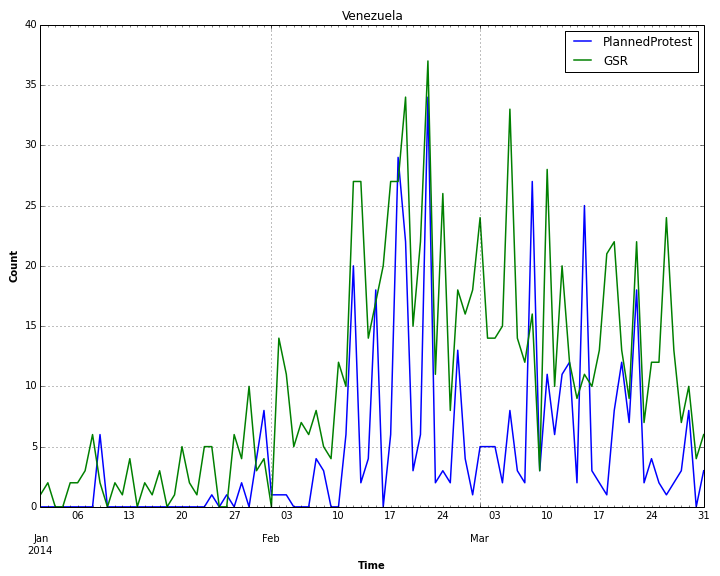
\includegraphics[width=\textwidth]{venezuela.png}
%        \caption{Venezuelan Protests}
%        \label{fig:Venezuela_feb}
%    \end{subfigure}
%    \begin{subfigure}[b][0.3\textwidth]
%        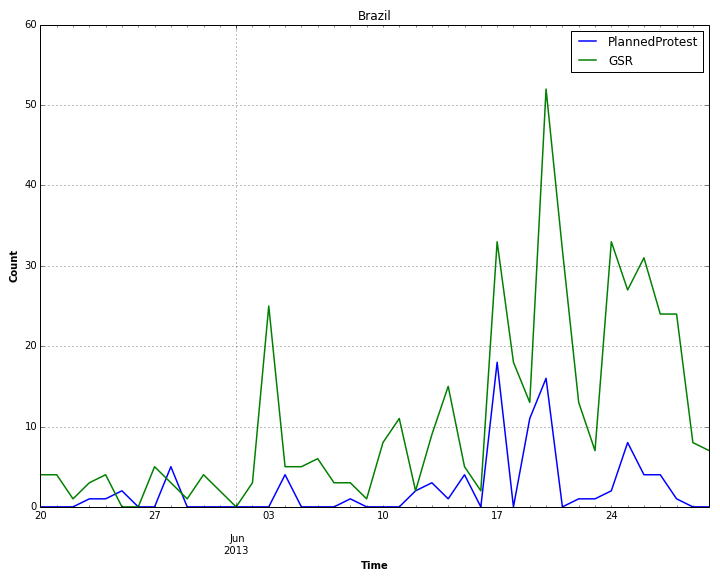
\includegraphics[width=\textwidth]{brazil_june.png}
%        \caption{Brazilian Riots in June}
%        \label{fig:Brazil_june}
%    \end{subfigure}
%\end{figure}
